\section{Theoretische Grundlagen}

\newcommand{\VG}{V_{\mathbf{G}}}
\newcommand{\G}{\mathbf{G}}
\newcommand{\g}{\mathbf{g}}
\newcommand{\R}{\mathbf{r}}
\newcommand{\K}{\mathbf{k}}
\newcommand{\A}{\mathbf{a}}
\newcommand{\ex}{\mathbf{e}^}

\subsection{Charakterisierung von Kristallgittern}
Vor der Beschreibung der Oberflächen von Kristallen wenden wir uns dem darunter liegenden 
Gitter zu, das die Basis für die Oberfläche darstellt. Die charakteristischen Größen 
sind auch für die Oberflächen wichtig. Die Untersuchung der Kristallgitter findet vor 
Allem durch Beugungsexperimente statt, da diese die periodische Struktur am besten 
Ausnutzen und so zu höherer Genauigkeit kommen, als direkte Abbildung der Oberflächen. 

Fundamental für die Beschreibung der Phänomene der Festkörperphysik ist der reziproke 
oder $\K$-Raum. Er ist aus den $\K$-Vektoren ebener Wellen, die mit 
$\ex{i \K \cdot \R}$ beschrieben werden, aufgebaut. Sind nun 
die Gittervektoren eines Kristalles im Ortsraum mit $\A_1,\ \A_2,\ \A_3$ gekennzeichnet, 
so gilt für die reziproken Gittervektoren $\g_1,\ \g_2,\ \g_3$:
\begin{eqnarray}
    \g_1 = 2 \pi \frac{\A_2 \times \A_3 }
        {\A_1\cdot (\A_2 \times \A_3)} \qquad \mathrm{und \ zyklisch} \\
    \mathbf{g_i} \cdot \mathbf{a_j} = 2 \pi \delta_{ij}
\end{eqnarray}
Die periodische Struktur des Kristalles bleibt also im reziproken Raum erhalten.
Ein beliebiger Vektor $\G$ des reziproken Gitters lässt sich als ganzzahlige Linearkombination 
der Basisvektoren darstellen.
\begin{equation}
    \mathbf{G} = h \mathbf{g_1} + k \mathbf{g_2} + l \mathbf{g_3}
\end{equation}
Für einen Vektor $\R$, der auf dem Gitter im Ortsraum liegt, gilt dann also:
\begin{eqnarray}
    \mathbf{r} &=& n_1 \mathbf{a_1} + n_2 \mathbf{a_2} + n_3 \mathbf{a_3} \\
    \mathbf{G} \cdot \mathbf{r}&=& 2 \pi m  \\
    n_1, \, n_2, \, n_3, \, m &\in& \mathbb{N}
\end{eqnarray}

Schließlich lässt sich jede Funktion, die im Ortsraum periodisch ist, als 
Fourierreihe im reziproken Raum darstellen:
\begin{equation}
    f(\R) = \sum_{\G} F_{\G} \ex{i \G \cdot \R}
\end{equation}

Bei der Bezeichnung der Netzebenen werden die sogenannten Millerschen Indizes benutzt. 
Spannt man mit drei nicht auf einer Geraden liegenden Gitterpunkten eine Ebene, so ist 
diese durch 
drei ganze Zahlen $m, n, o$ gekennzeichnet. Aus diesen erhält man ein teilerfremdes 
Triplet $(h, k, l)$, indem man die reziproken Werte $h' = 1/m, k' = 1/n, l' = 1/o$ mit 
einer ganzen Zahl $p$ multipliziert. Der reziproke 
Gittervektor $\G$ steht nun senkrecht auf dem mit $(h, k, l)$ beschriebenen Gitter.
\cite{ibach2009festkorperphysik}


\subsection{Blochtheorie und Bändermodell}

Für die Rastertunnelmikroskopie ist die räumliche Verteilung der Elektronen an 
der Oberfläche von zentraler Bedeutung. Die Blochtheorie macht Aussagen über 
die Aufenthaltswahrscheinlichkeiten von Elektronen in periodischen 
Gittern und liefert ein Modell zur Erklärung des Bändermodells. 
Für ein Elektron mit Wellenfunktion $\psi$ gilt bei Vernachlässigung der 
Elektron-Elektron-Wechselwirkung in der nichtrelativistischen Näherung die 
Schrödingergleichung 
\begin{equation}
    \hat H \psi(\R) = \Big[ - \frac{\hbar^2}{2m} \Delta + V(\R) \Big] \psi(\R) = E \psi(\R)
\end{equation}
mit periodischem Potential
\begin{equation}
    V(\R) = V(\mathbf{r + r_n}); 
\qquad \mathbf{r_n} = n_1 \mathbf{a_1} + n_2 \mathbf{a_2} + n_3 \mathbf{a_3} 
\end{equation}
wobei $\mathbf{a_i}$ Gittervektoren des Ortsraumes sind. Auf Grund der Periodizität lässt 
sich das Potential in eine Fourierreihe zerlegen:
\begin{eqnarray}
    V(\R) &= &\sum_\G \VG \mathrm{e}^{i\G \cdot \R} \\
    \mathrm{mit \ Fourierkomponente \quad}  \VG &= &\frac{1}{L} \int \mathrm{e}^{i\G \cdot \R} 
    V(\R) \mathrm{d}\R  \nonumber \\
    \mathrm{und \ reziprokem \ Gittervektor \quad} \G &= &h\mathbf{g_1} + k\mathbf{g_2} +l\mathbf{g_3}; 
    \quad h, \ l, \ k, \ \in \mathbb{Z}. \nonumber
\end{eqnarray}

Der Ansatz für die Lösung ist eine Linearkombination ebener Wellen
$ \psi(\R) = \sum_\K C_\K \mathrm{e}^{i\K \cdot \R}, $
für die nach Einsetzen in die Schrödingergleichung gelten muss:
\begin{equation}
    \sum_\K \mathrm{e}^{i\K \cdot \R} 
    \Big[ \Big( \frac{\hbar^2 k^2}{2m} - E\Big) C_\K + \sum_\G \VG C_{\K - \G}\Big] 
    = 0
\end{equation}
Aus der Unabhängigkeit von $\R$ folgt dann
\begin{equation}
    \Big( \frac{\hbar^2 k^2}{2m} - E\Big) C_\K + \sum_\G \VG C_{\K - \G}= 0
\end{equation}

Zu jeden $\K$ Wert ergeben sich also $N$ Gleichungen, die die Koeffizienten
$C_\K$ jeweils mit $C_{\K - \G'}$, $C_{\K - \G''}$,\ldots  koppeln, wobei $N$ die Anzahl 
der Elementarzellen im Gitter ist. Daher lassen sich die Wellenfunktionen 
mit Energie $E_\K$ also Superposition ebener Wellen schreiben, deren $\K$ Werte 
alle auf dem reziproken Gitter liegen: 

\begin{eqnarray}
    \psi_\K(\R)&=& \sum_\G C_{\K - \G} \mathrm{e}^{i(\K - \G) \cdot \R} \nonumber \\
            &=& \sum_\G C_{\K - \G} \mathrm{e}^{i \G \cdot \R}  \mathrm{e}^{i\K \cdot \R} \nonumber \\
            &=& u_\K(\R) \cdot \mathrm{e}^{-i\K \cdot \R} 
\end{eqnarray}

Diese Wellenfunktionen werden Bloch-Wellen genannt. Das Bloch-Theorem sagt aus, 
dass für das Einelektronenproblem im periodischen Potential eben diese Bloch-Wellen 
Energie-Eigenfunktionen mit Eigenwerten $E_\K$ mit $\K = \frac{2 \pi}{L} (n_x, n_y, n_z)$ und
\begin{equation}
    u_\K(\R) = u_\K(\mathbf{r + r_n}) 
\end{equation}
sind. Es folgt direkt 
\begin{equation}
    \psi_{\K + \G}(\R) = \psi_\K(\R) 
\end{equation}
und damit auch: 
\begin{equation}
    E(\K) = E(\K + \G)
\end{equation}
Für die Aufenthaltswahrscheinlichkeit folgt $|\psi(\mathbf{r})|^2 = |u|^2$ - wir können also 
die Elektronendichte als Messgröße für die Positionen der Atomrümpfe verwenden!

Mit Hilfe der Näherung für ein quasifreies Elektron liefert die Bloch-Theorie auch einen 
Ansatz für die Erklärung der Bänderstruktur in Festkörpern. Dafür gehen wir von einem freien 
Elektron aus, für das jedoch weiter die Periodizität im Raum gelten soll (das sog. \emph{'leere Gitter'}). 
Verschieben wir nun unser Gitter um einen reziproken Gittervektor $\G$, so ließt sich die 
Schrödingergleichung im $\K$-Raum wie folgt:
\begin{eqnarray}
    \Big(E - \frac{\hbar^2}{2m}|\K - \G|^2\Big) C_{\K - \G} &=&
        \sum_{\G'} V_\mathbf{G' - G} C_{\K - \G'}, \quad \mathrm{d.\ h.} \nonumber \\
    \label{eqn:bloch1}    
    C_{\K - \G} &=& \frac{ \sum_{\G'} V_\mathbf{G' - G}}{E - \frac{\hbar^2}{2m}|\K - \G|^2} 
\end{eqnarray}


Gehen wir nun von einer Störung des Falles eines freien Elektrons aus, so können wir 
die eigentliche Energie in erster Näherung durch $E = (\hbar^2 k^2) / (2m)$ ersetzen. 
Da wir nur die größten Koeffizienten $C$ betrachten, sollte der Nenner 
in \eqref{eqn:bloch1} möglichst klein werden, es sollte also die Beziehung 
\begin{equation}
    E(\K) = E(\K + \G)
\end{equation}
gelten, die genau die Braggbedingung für Reflexion ist. D.~h. die stärkste Abweichung zum freien 
Elektron treten dann auf, wenn der $\K$ Vektor auf dem Rand der sog. \emph{1. Brillouin-Zone} liegt. 
Weiterhin folgt mit $V_0 = 0$ durch einsetzen von $\G = 0$ in \eqref{eqn:bloch1}, dass auch $C_\K$ in der ersten Ordnung 
beträgt. Daher ergibt sich das Gleichungssystem 
\begin{eqnarray}
    \psi_\K(\R)&=& \sum_\G C_{\K - \G} \mathrm{e}^{i(\K - \G) \cdot \R} \nonumber \\
            &=& \sum_\G C_{\K - \G} \mathrm{e}^{i \G \cdot \R}  \mathrm{e}^{i\K \cdot \R} \nonumber \\
            &=& u_\K(\R) \cdot \mathrm{e}^{-i\K \cdot \R} 
\end{eqnarray}

welches die Determinantengleichung 
\begin{eqnarray}
    \begin{vmatrix}
        \Big(\frac{\hbar^2}{2m} k^2 - E\Big) & \VG \\
        V_\mathbf{-G}   & \Big(\frac{\hbar^2}{2m} |\K - \G|^2 - E\Big) 
    \end{vmatrix} = 0; \\
    E_{\K - \G}^0 = \frac{\hbar^2}{2m} |\K - \G|^2 \nonumber
\end{eqnarray}
mit den Lösungen 
\begin{equation}
    E^\pm = 
    \frac{1}{2}(E_{\K - \G}^0 + E_\K^0) \pm 
        \frac{1}{2}\Big[(E_{\K - \G}^0 + E_\K^0)^2 + |\VG|^2\Big]^{\frac{1}{2}}
\end{equation}

auflöst. Unmittelbar auf dem Rand der 1. Brillouin-Zone gilt $E_{\K - \G}^0 = E_\K^0$ und 
damit für die Energiedifferenz der Bänder: 
\begin{equation}
    \Delta E = E^+ - E^- = 2 |\VG|
\end{equation}
Für den eindimensionalen Fall ist das in Abb.~\ref{fig:bloch} schematisch dargestellt.
\cite{ibach2009festkorperphysik} 

\begin{figure}[!t]
  \begin{captionbeside}[]{Darstellung der Aufspaltung der Energieparabel des freien Elektrons 
(gestrichelt) an den Rändern der 1. Brillouin-Zone im Rahmen der störungestheoretischen 
Betrachtung von Elektronen in periodischen Gittern (hier für den eindimensionalen Fall). 
(1) und (2) markieren die jeweiligen Bänder. 
Aus \cite{ibach2009festkorperphysik}.}[r]
    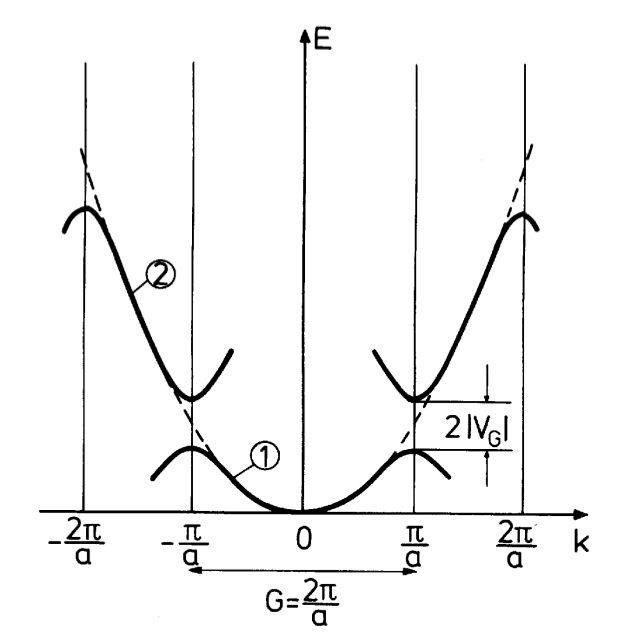
\includegraphics[width=0.5\textwidth]{pics/bloch}
  \end{captionbeside}
  \label{fig:bloch}
\end{figure}

Im Kristall gibt es nun Abweichungen von dem Modell. Zuerst einmal haben Kristalle 
endliche Ausdehnungen, sodass das zuvor als kontinuierlich angenommene 
Energiespektrum diskret ist. Zweitens haben die Elektronen eine Wechselwirkung. 
Diese ist gering im Vergleich zum Potenzial der Kerne, allerdings sorgt sie dafür, 
dass sich die erlaubten Energiewerte für Elektronen eines einzelnen Atoms aufspalten 
in $N$ sehr nahe beieinander liegenden Werten. Für große $N$ sind die erlaubten 
Energiewerte in dem so entstandenen \emph{Band} nahezu kontinuierlich, 
siehe Abb.~\ref{fig:baender1}. Pro Band können  
sich nach dem Pauliprinzip und unter Berücksichtigung des Spins maximal 2N Elektronen 
befinden. Geht die Temperatur gegen Null, so sind die Elektronen in der Konfiguration 
mit der niedrigsten möglichen Gesamtenergie angeordnet. Das oberste dann voll mit 
Elektronen besetzte Band wird als \emph{Valenzband} bezeichnet. Wird die Temperatur 
erhöht, so steht thermische Energie zu Verfügung. Die maximal Energie, die Elektronen 
im Mittel erhalten würden, wenn erlaubte Energiezustände vorhanden wären, wird als 
\emph{Fermienergie} bezeichnet. 
Liegt das Energieband über dem Valenzband unterhalb der Fermienergie oder hat sogar 
einen Überlapp mit dem Valenzband, so können Elektronen Enrgie aufnehmen und in dieses 
Band gelangen. Dort sind sie räumlich deutlich schwächer gebunden und können bei einem 
von außen angelegtem Feld in Richtung des Feldes driften. Daher wird das Band über dem 
Valenzband als \emph{Leitungsband} bezeichnet. Metalle sind deshalb elektrische Leiter, weil 
bei ihnen Leitungs- und Valenzband überlappen. Für das einwertige Natrium ist beispielsweise 
das oberste besetzte Band, das sich aus den 3$s$-Orbitalen zusammensetzt, nur halb besetzt. 
Für zweiwertige Metalle wie Magnesium überlappen sich Leitungs- und Valenzband. 
Bei Isolatoren liegt die Fermienergie niedriger als die untere Kante des Leitungsbandes. 
Die Elektronen können keine Energie eines angelegten Feldes aufnehmen und es kann kein 
Strom fließen. Bei Halbleitern ist die Fermienergie ab einer bestimmten Energie höher 
als die niedrigste Energie des Leitungsbandes. Daher ist ihre Leitfähigkeit 
temperaturabhängig. Siehe Abb.~\ref{fig:baender2}.\cite{demtroder2000experimentalphysik}\\ 

\newcommand{\picwidththeo}{0.48\textwidth}

\begin{figure}
    \centering
    \begin{subfigure}[b]{\picwidththeo}
        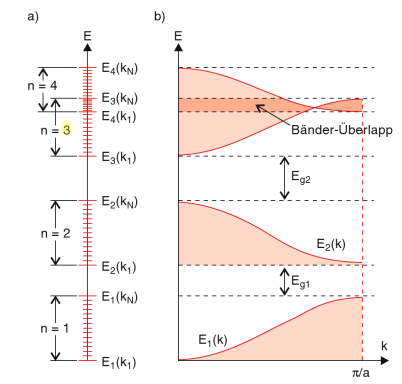
\includegraphics[width=\textwidth]{pics/baender1}
        \caption{Zur Entstehung der Energiebänder. Dargestellt ist die Aufspaltung der erlaubten 
Energiewerte von $N$ Elektronen im Kristall. 
(a) Eindimensionale Darstellung, 
(b) Darstellung von $E_n(k)$, die gestrichelte Linie ist die Grenze der 1. Brillouin-Zone;
aus \cite{demtroder2000experimentalphysik}}
        \label{fig:baender1}
    \end{subfigure}\qquad
    \begin{subfigure}[b]{\picwidththeo}
        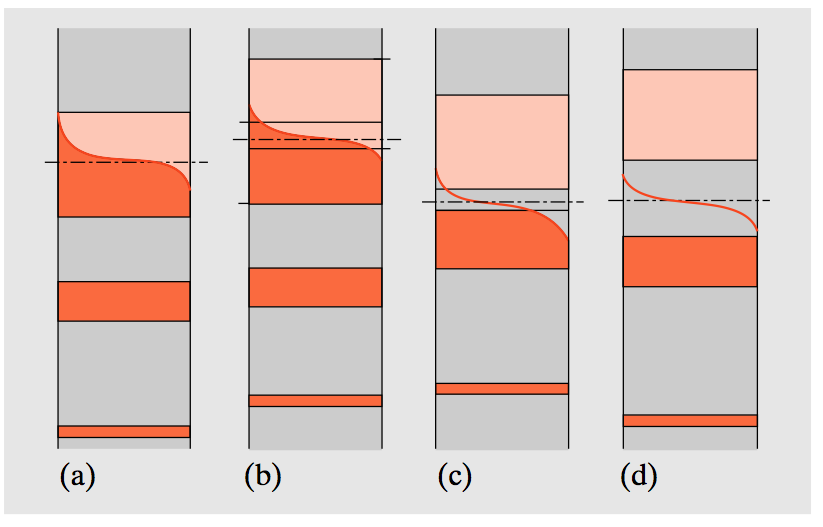
\includegraphics[width=\textwidth]{pics/baender2}
        \caption{Vereinfachte Darstellung des Bändermodells für 
(a) Metalle der ersten Hauptgruppe (Alkalimetalle), 
(b) Metalle der zweitern Hauptgruppe (Erdalkalimetalle), 
(c) Halbleiter (im leitfähigen Zustand)
(d) Isolatoren
aus \cite{vogel1997gerthsen}}
        \label{fig:baender2}
    \end{subfigure}
    \caption{Schemata zum Bändermodell}\label{fig:baender}
\end{figure}



\subsection{Grundlagen der Festkörperoberflächen}
Das zuvor angenommen, unendlich ausgedehnte, periodische Kristallgitter spielt 
bei der Untersuchung der Oberflächen nur noch eine untergeordnete Rolle – 
schließlich ist eine Oberfläche zunächst einmal eine Abweichung dieser 
Eigenschaft. Im Allgemeinen kann es Abweichungen in null, ein, zwei oder drei 
Dimensionen geben. Letztere sind Abweichungen der unterliegenden Baustruktur, 
die zum Teil eine Mosaikstruktur bilden, die sich auch auf größere Skalen 
erstrecken. Zweidimensionale Strukturen tauchen als großflächige 
Überstrukturen oder kleinere Facetten auf. Eine Kategorisierung verschiedener 
Oberflächen wird von Henzler und Göpel \cite{henzler1991oberflachenphysik} 
gegeben (Abb.:~\ref{fig:oberflaeche}).
In jedem Fall erfahren die Atome der Oberfläche erfahren nicht mehr das 
regelmäßige Potential von allen Seiten. Die resultierenden Veränderung werden je 
nach Art als Oberflächenrelaxation oder -rekonstruktion. 
Ersteres bezeichnet lediglich eine globale Verschiebung der oberen Schicht 
gegen die Basis, beispielsweise normal oder lateral, wobei die Symmetrien 
der Oberfläche nicht verändert werden und sich die freie Energie verringert. 
Dieser Effekt wird bei den meisten Metallen beobachtet \cite{oura2003surface}. 
Abb. \ref{fig:Ag(110)} zeigt beispielsweise die relaxierte Oberfläche von Silber 
auf der (110)-Fläche.
Bei der Oberflächenrekonstruktion bilden sich meist größere Einheitszellen, als die 
des darunter liegenden Kristalls. Bei Halbleitern hängt das oft damit zusammen, 
dass die Anzahl nicht abgesättigter Bindungen minimiert wird, so beispielsweise 
bei Silizium entlang der (100)-Fläche, bei der nach gedanklichem Aufspalten zwei 
Bindungen frei wären. Je zwei Atome verbinden sich zu sog. Dimeren, wobei die 
Oberfläche räumlich verzogen wird und sich volle bzw. leere Reihen mit einer 
Höhe von bis zu fünf Schichten und über große Entfernungen bilden 
\cite{chadi1979atomic}. Die bereits in der historischen Einleitung gezeigte 
Si-Oberfläche entlang der 
(111)-Ebene zeigt ebensfalls eine Oberflächenrekonstruktion, allerdings mit 
deutlich anderen Mustern. Die kubisch-flächenzentrierten Edelmetalle der 
6.~Periode, Ir, Pt und Au bilden als Ausnahme unter den Metallen ebenfalls 
Oberflächenrekonstruktionen, die sog. \emph{missing row}-Konstruktion, 
wie weiter unten bei der Beschreibung von Gold verdeutlicht wird 
\cite{kittel2013einfuhrung}. 

\begin{figure}[!t]
  \begin{captionbeside}[]{Rastertunnelkikroskop-Aufnahme mit atomare Auflösung einer reinen 
Silberoberfläche entlang der (110)-Fläche. Zu erkennen ist, dass die Oberfläche 
lediglich relaxiert ist, und Rekonstruktion stattfindet. 
Aus \cite{kahn:stm_images}.}[r]
    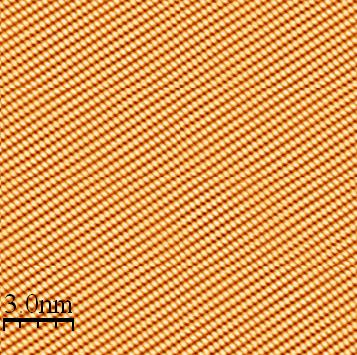
\includegraphics[width=0.5\textwidth]{pics/Ag(110)_clean}
  \end{captionbeside}
  \label{fig:Ag(110)}
\end{figure}

Zur mathematischen Beschreibung regelmäßiger Überflächen werden die Gittervektoren 
aus dem Ortsraum benutzt, die in der Oberfläche liegen. Ausreichend sind meistens 
jene aus der obersten Atomschicht. Die Atome befinden sich dann an den Positionen 
\begin{equation}
    \mathbf{r} = m_1 \mathbf{a_1} + m_2 \mathbf{a_2},
\end{equation}
wobei nach Konvention $|\mathbf{a_1}| \le |\mathbf{a_2}|$ und 
$\gamma = \angle (\mathbf{a_1}, \mathbf{a_2}) > 90 \deg$ der Winkel zwischen den 
beiden Vektoren ist. Da die Atom in einer Ebene liegen, ist die Anzahl möglicher 
Anordnungen, die sog. Bravais-Netze, deutlich kleiner als für einen 3D-Kristall. 
Es gibt genau fünf, wie in Abb.~\ref{fig:Bravais} gezeigt 
\cite{henzler1991oberflachenphysik}.
Zur vollständigen Beschreibung fehlen dann allerdings noch die Angaben zur Lage 
der Oberflächenatome relativ zur darunter befindlichen Basis. 

Zur Beschreibung der Oberfläche wird zuerst die ideale Oberfläche angenommen, 
die sich aus dem darunter liegenden Kristallgitter ergäbe, und deren Vektoren mit
$|\mathbf{a_1}| \le |\mathbf{a_2}|$ bezeichnet werden. Die tatsächle Struktur, 
soweit periodisch, kann dann als Verhältnisse $\frac{\mathbf{a_1}}{\mathbf{b_1}}$, 
$\frac{\mathbf{a_1}}{\mathbf{b_1}}$ und Winkel zwischen Basis und Oberfläche angegeben 
werden. Zusammen mit der Millerschen Schreibweise für die Kristallfläche der Basis 
ergibt sich so eine kompakte Schreibweise, z.~B. 
$\mathrm{Si}(111)(\sqrt{3} \times \sqrt{3}) \mathrm{R} 30 \deg$. 
Ist diese Schreibweise ungeeignet aufgrund fehlender Symmetrien, so kann eine 
Matrixschreibweise benutzt werden. Sind die Einträge ganze Zahlen, so liegen die 
Atome der Oberfläche direkt auf der Basis. Bei rationalen Zahlen gibt es auch 
zwischen den Basisatomen Oberflächenatome, während bei irrationalen Zahlen die 
Oberfläche quasi unabhänging von der Basis gesehen werden muss. Sie wird dann auch 
als inkommensurabel bezeichnet. \cite{henzler1991oberflachenphysik}

\begin{figure}
    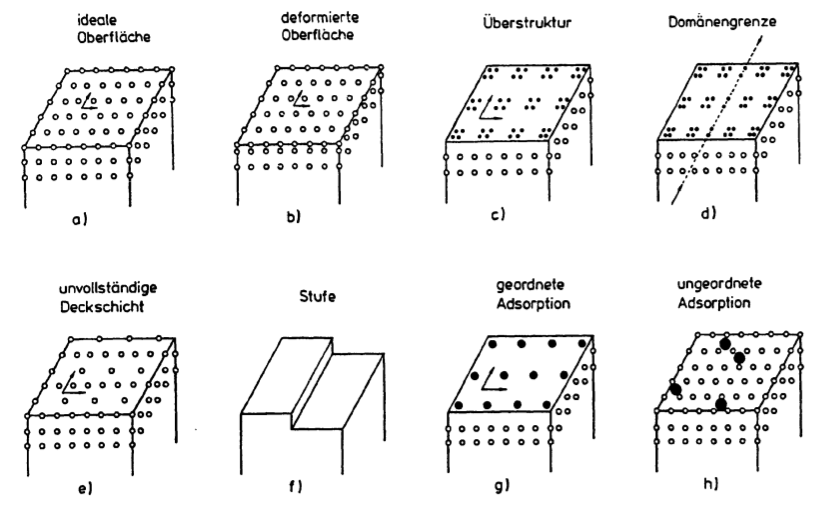
\includegraphics[width=1.0\textwidth]{pics/oberflaechenstruktur}
    \caption{Die ideale Oberfläche und einige mögliche Oberflächenstrukturen. 
Die ideale Oberfläche entspricht einer Gitterebene im Kristall, die defomierte 
Oberfläche entsteht durch Relaxation (hier in normaler Richtung) und wird bei den 
meisten Metallen beobachtet, während die Überstruktur ein Resultat der Rekonstruktion 
ist und z. B. bei Halbleitern oder Gold zu beobachten ist. 
Aus \cite{henzler1991oberflachenphysik} }
    \label{fig:oberflaeche}
\end{figure} 
\begin{figure}
  \begin{captionbeside}{Bravais-Gitter zur Oberflächenstrukturbeschreibung. Die 
kleinstmöglichen Zellen sind in den unteren drei Gittern mit $\underline{a}_2^p$ 
beschriftet. 
Aus \cite{henzler1991oberflachenphysik}.}[r]
    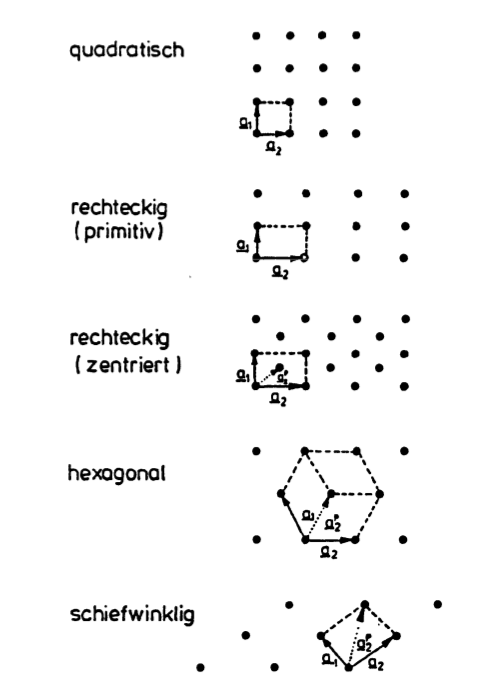
\includegraphics[width=0.5\textwidth]{pics/Bravais}
  \end{captionbeside}
  \label{fig:Bravais}
\end{figure} 


\subsection{Struktur von Graphit, Gold und $\mathrm{MoS_2}$}
Die Kristallstruktur von Graphit zeichnet sich vor allem durch seine Schichtenstruktur 
aus. Die Kohlenstoffatome sind in den aus kovalent gebundenen Sechsecken bestehenden 
Basalebenen oder Graphenschichten deutlich fester aneinander gebunden (4.3 eV), als 
an solche aus benachbarten Schichten (0.07 eV). Daher ist Graphit entlang dieser Linien 
sowohl mechnisch deutlich stabiler als auch sehr viel leitfähiger (für Wärme und 
elektrischen Strom). Die Unterschiede in der Bindungsenergie spiegeln sich auch in den 
Abständen wider: So sind nächsten Nachbarn innerhalb einer Schicht nur $0.142\mathrm{nm}$ 
entfernt, während die Schichten $0.335\mathrm{nm}$ auseinander liegen.  
Graphit tritt nicht nur in zueinander korrlierten Schichten auf, 
sondern auch unkorrliert (sog. turbostratischer Kohlenstoff). Die hier untersuchte Form 
ist jedoch regelmäßig - die Winkelabweichung für das verwendete HOPG (highly orientated 
pyrolytic graphite) beträgt weniger als $1 \deg$ \cite{mcnaught2000iupac}. Diese 
synthetische Form des Graphit wird auf Grund von ihrer Regelmäßigkeit und Reinheit 
heute zur Kalibrierung von Rastertunnelmirkoskopen verwendet \cite{lapshin1998automatic}. 
Es liegen in der Schichtung jedoch nicht alle Atome übereinander, sondern lediglich 
jedes zweite aus jedem Sechseck (siehe Abb.~\ref{fig:graphite}). 
Dadurch kommt es an der Oberfläche zu einem oft beobachteten 
Effekt: Anstatt sämtliche Atome der Sechsecke zu beobachten, taucht nur die Hälfte auf 
den STM-Bildern auf. Erklärt wird das dadurch, dass die Elektronendichte in der 
Fermienergie für Atome mit Nachbarn darunter höher liegt als bei solchen ohne
\cite{zeinalipour2008new}. Selloni~et~al.~\cite{Sellino1985} berechneten den Abstand 
der Atome mit bzw. ohne direkten Nachbarn in der Schicht darunter mit $0.15 \AA$. 

\begin{figure}
    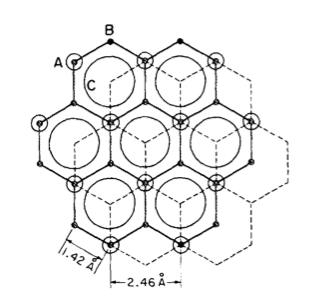
\includegraphics[width=0.7\textwidth]{pics/graphite}
    \caption{Hexagonale Oberflächenstruktur von Graphit. An den umkreisten Orten (A) 
liegen jeweils Atome aus der ersten und der zweiten Schicht übereinander, bei den 
übrigen (B) nicht. Bei STM-Aufnahmen sind fast ausschließlich die Atome mit Nachbarn 
zu erkennen, da hier Elektronen nahe der Fermienergie räumlich weiter oben liegen. 
Aus \cite{park1986tunneling}}
    \label{fig:graphite}
\end{figure} 

Gold ist als kubisch-flächenzentriertes Kristallgitter aufgebaut. Die Gitterkonstante 
beträgt $407.82\mathrm{pm}$\cite{ohring1995engineering}. Im Gegensatz zum Graphit 
treten jedoch beim Gold enorme Veränderungen der Oberflächenstruktur gegenüber der 
darunter liegenden Basis auf. Auf einer (110)-Fläche wurde die Bildung von 
(111)-Facetten beobachtetet, die Kanälevon meistens zwei bis vier Schichten Tiefe 
formen. Gleichzeitig ist die Oberfläche von Stufen gekennzeichnet, die sowohl parallel 
als auch normal zu den Kanälen verlaufen, siehe Abb. \ref{fig:Au(110)_channels}. Die Darstellung 
der Oberfläche mit dem Rastertunnelmikroskop ist auf Grund der metallischen Struktur 
deutlich schwieriger als bei Halbleitern, da die Elektronen aus dem Leitungsband kaum 
räumlich lokalisiert sind. 

\begin{figure}
    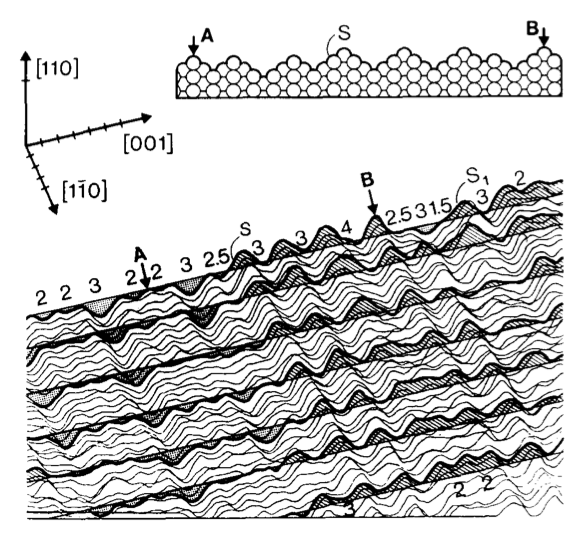
\includegraphics[width=0.6\textwidth]{pics/Au(110)_channels}
    \caption{Rastertunnelmikroskop-Aufnahmen von Gold(110)-Oberfläche mit 
Rekonstruktion. Die Geraden verdeutlichen die abschüssige Terassenstruktur, die 
Nummern die Tiefe der Kanäle (in Vielfachen der Ebenenabstände). Bei $\mathrm{S}$
und $\mathrm{S_1}$ befinden sich Stufen mit Höhe einer Atomlage. An den Kristallaxen 
ist der Maßstab gekennzeichnet: ein Schritt entsprechen 5 \AA. Über der Aufnahme 
deutet ein schematischer Querschnitt die Struktur der Kanäle an. 
Aus \cite{binnig1983111}.}
    \label{fig:Ag(100)}
\end{figure} 

Molybdänit ($\mathrm{MoS_2}$, auch Molybdän(IV)-sulfid) ist ein Halbleiter mit 
hexagonalem Kristallgitter der Raumgruppe $\mathrm{P \, 6_3/mmc}$. Ähnlich 
dem Graphit gibt es eine schichtartige Struktur, auch hier können die Schichten 
relativ leicht gegeneinander verschoben werden. Die Gitterparameter sind mit 
$a = 3.161 \AA$ sowie $c = 12.295 \AA$ angegeben, siehe
Abb.~\ref{fig:MoS2_structure} \cite{schrocke1981mineralogie}. 
Auf Gund der Schichtstruktur findet $\mathrm{MoS_2}$ als 
Schmiermittel Verwendung und kann wie Graphen als einatomige Schicht isoliert 
werden, sodass es mögliches Transitormaterial gehandelt wird 
\cite{mak2010atomically}. 

\begin{figure}
  \begin{captionbeside}{Gitterstruktur von $\mathrm{MoS_2}$, Ausschnitte aus drei übereinander 
liegenden Schichten mitsamt Koordinationspolyedern. Für die Abstände gilt 
$a_1 = a_2 = a_3 = 3.161\AA =: a$ und $c_0 = 12.295\AA$. 
Aus \cite{schrocke1981mineralogie}.}[r]
    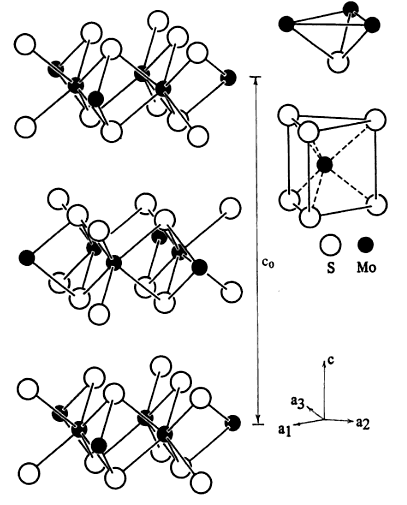
\includegraphics[width=0.5\textwidth]{pics/MoS2_structure}
  \end{captionbeside}
  \label{fig:MoS2_structure}
\end{figure} 
